Pusteblume ist der Kosename für den Löwenzahn, auch \textit{Taraxacum (officinale)} genannt.
Hierbei handelt es sich um Pflanzen der Familie der Korbblütler,
die \enquote{weltweit von den Tropen bis zu den Polargebieten verbreitet}\footfullcite{Taraxacum} auffindbar sind.\\

\noindent
Ihren globalen Erfolg haben sie vor allem ihrer Fortpflanzung zu bedanken,
denn sie sind fähig sich asexuell zu vermehren, und können pro Pflanze bis zu 20.000 Diasporen, die jeweils kilometerweit fliegen können, erzeugen.\footfullcite{wisc-dandelion}\footcite{Taraxacum}


\begin{figure}[h]
    \centering
    \begin{minipage}{0.45\textwidth}
        \centering
        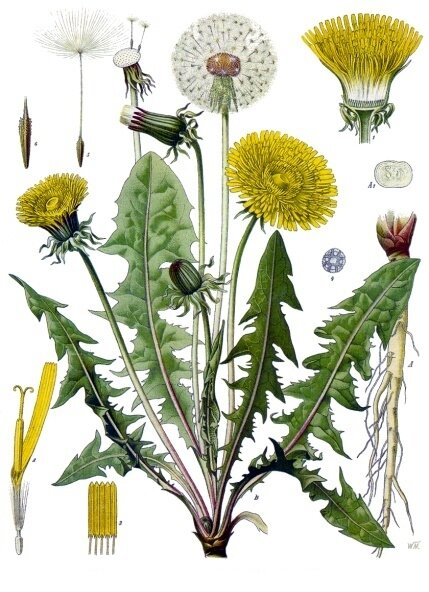
\includegraphics[width=\textwidth]{Drawing-representing-the-life-cycle-of-Taraxacum-officinale-2}
        \caption{Taraxacum officinale\cite[, Fig 2.1]{tesi}}
    \end{minipage}
    \hfill
    \begin{minipage}{0.5\textwidth}
        \centering
        \setbox0\hbox
        {\includegraphics[width=\textwidth]{achäne-schema}}
        \ht0=10cm % change this to move it up or down
        \dp0=0cm
        \box0
        \caption{Eine Achäne \cite[\textit{in Anlehnung an}][, Fig 1.1]{tesi}}
        \label{fig:figure3}
    \end{minipage}
\end{figure}

\newpage

\subsection{Achäne}\label{subsec:achane}

Wie in Abbildung ~\ref{fig:figure3} veranschaulicht besteht die Achäne - die Diaspore des \textit{Taraxacum officinale} hauptsächlich aus Pappus und Samen.
Die Härchen des Pappus haben mikroskopische Dornen die radial aus den Härchen hervortreten,
und bestehen, ähnlich wie Holz, aus hohlen Röhrchen.\footfullcite{morph}
Diese Konstruktion verleiht den Härchen stabilität und ein geringes Gewicht.

\begin{figure}[h]
    \centering
    \begin{minipage}{0.4\textwidth}
        \centering
        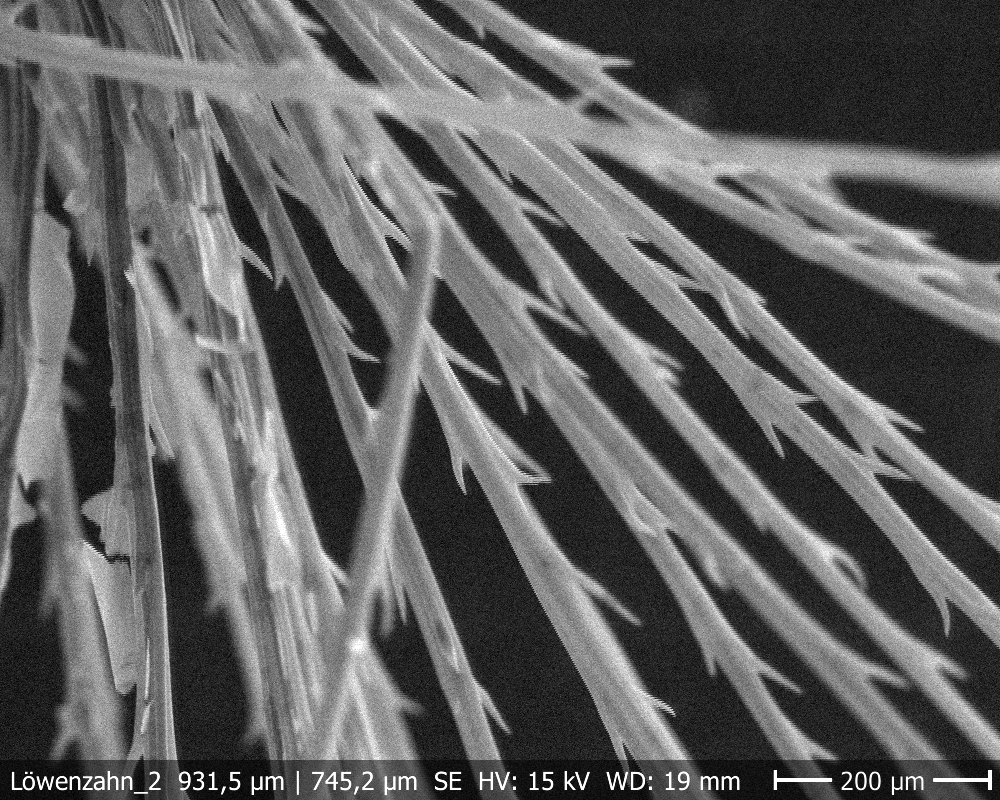
\includegraphics[width=\textwidth]{sam_pusteblume_2}
        \caption{Elektronenmikroskopie der Pappushärchen, [\textit{Eigene Darstellung}]}
        \label{fig:emk_1}
        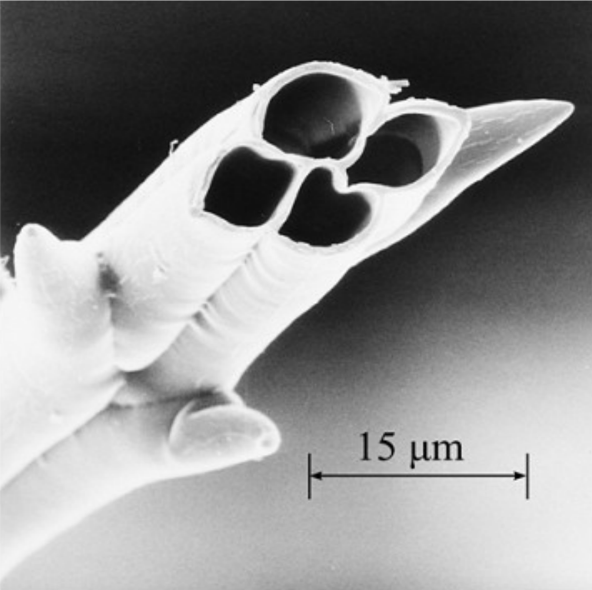
\includegraphics[width=0.8\textwidth]{Pappushaar}%
        \caption{Elektronenmikroskopie der Pappushärchen, \cite[, Fig. 9]{morph}}
        \label{fig:emk_2}
    \end{minipage}
    \hfill
    \begin{minipage}{0.3\textwidth}
        \centering
        \includegraphics[width=\textwidth]{Fallverhalten_achäne}%
        \caption{Fallverhalten der Achäe, \cite[, Fig. 4]{morph}}
        \label{fig:flt}
    \end{minipage}
\end{figure}

Die Positionierung des Samens bewirkt einen tiefen Schwerpunkt vom Flugkörper.
Dadurch richtet er sich im Flug, sodass der Samen unten, und der Pappus oben,
und senkrecht zur Fallrichtung ausrichtet ist, wie in Abbildung ~\ref{fig:flt}.\\
\enquote{Der Pappus [...] fungiert als Fallschirm und ist die Ursache der relativ langsamen Fallgeschwindigkeit.}\footfullcite[(Übersetzt)]{morph}

\newpage